% Activate the following line by filling in the right side. If for example the name of the root file is Main.tex, write
% "...root = Main.tex" if the chapter file is in the same directory, and "...root = ../Main.tex" if the chapter is in a subdirectory.
 
%!TEX root =  dissertation.tex

\chapter[Design \& Implementation]{Design \& Implementation}

In this chapter, I will discuss HemeWeb's development and implementation. This will consist on how the HemeLB core Docker container is developed, how it is deployed, and how the web application is developed.


\section{HemeLB core Docker container}

HemeLB core is a Docker container that consists of essential software and services needed to run HemeLB simulation. It is the main component that runs the HemeLB simulation on the cloud. Calculations will be done on the container which will be started on the compute nodes of the HemeWeb architecture. 

Previously, there was an effort to make HemeLB software package portable by creating its own container package\footnote{\url{https://github.com/mobernabeu/docker-hemelb}}. It has all the necessary tools for HemeLB simulation workflows such as setup tools, HemeLB binary, and post-processing scripts. Moreover, it also includes a Virtual Network Computing(VNC) capability that allows users to access the container's headless graphical user interface via HTML5 capable browser. All of these are necessary to make HemeLB more portable. Independent peers can replicate and reproduce simulation without having to configure all above tools. However, users will still need to configure Docker on their workstation to be able to run the container. HemeWeb will take this effort a step further. With HemeWeb, users will not be required to install any tools to run simulation workflows. Only web browser, which is normally installed by default, is needed.


In this phase, I took the previous container and modify the Dockerfile, the instructions file to build the container. The original Dockerfile uses a base image of Ubuntu\footnote{\url{http://www.ubuntu.com}}, a popular open source operating system, that is provided by Docker. This image by Docker incorrectly handle Ubuntu's init system, Upstart\footnote{\url{http://upstart.ubuntu.com}}, that results in some system services cannot be started correctly. One of this service is Secure Shell daemon(sshd)\footnote{\url{http://www.openssh.comm}}. This daemon is responsible for allowing remote users to get secure encrypted access to the host, in this case, a Docker container. Without sshd, HemeLB, which is a Message Passing Interface(MPI) application, cannot run a multi-host simulation because communication cannot be done between hosts.  To solve this issue, I switched the base image to base ubuntu provided by Phusion\footnote{\url{https://github.com/phusion/baseimage-docker#}}, a company in Netherland that open-sourced their version of Ubuntu container that solves above problem.

After switching the base image of the Docker container with Phusion's Ubuntu (Line 8 listing  \ref{lst:dockerfile}), I added commands to correctly start the ssh service, and configure the access keys. It is currently configured to use a shared insecure key that is committed to the repository. Ideally, this should be automatically generated at each container build, however, due to the  time limit of this project, this is not done yet. The next step is to strip out tools which will not be needed by the compute nodes to run HemeLB simulation. I added commands to purge the packages that are not essentials to the compute nodes. The resulting container is a minimal container that contains only the HemeLB binary and SSH service running. With these changes, the size of the container is also halved from originally 948MB\footnote{\url{https://hub.docker.com/r/mobernabeu/hemelb/tags/}} to 430 MB\footnote{\url{https://hub.docker.com/r/seiryuz/hemelb-core/tags/}}.


The modification of the Dockerfile of the container is the initial part to make HemeLB core container created correctly. To correctly create the HemeLB container, this Dockerfile needs to be integrated into the development workflow of HemeLB. Currently, the modified Dockerfile still live under the HemeWeb codebase\footnote{\url{https://github.com/SeiryuZ/HemeWeb/tree/master/hemelb_docker}}. HemeLB development should trigger an automated build of HemeLB core containers with each version of the software it pushes to the public GitHub repositories. In addition, the development team also needs to create a consistent tag naming in order for the HemeLB core containers to be created correctly.


\section{Deployment scripts}

The next step of the implementation is to develop deployment scripts to configure the overall software architecture. Due to the nature of the architecture that consists of many moving parts, manual configuration is not considered a manageable solution. I decided to create deployment scripts that alleviate the pain of deployment by provisioning and configuring the architecture with minimal manual intervention.  The scripts are created using a configuration management and orchestration tools called Ansible\footnote{\url{https://www.ansible.com}}.

Ansible is arguably the most popular tools in IT infrastructure automation space\citep{mohaan2014learning}. It is a python-based open source tool that is used for provisioning, configuring, and orchestration of IT infrastructure. Moreover, it is an agentless software that allows it to work without installing client-side software on the hosts it manages. I decided to use Ansible for deploying HemeWeb's infrastructure because it is developed in Python and also an agentless software\citep{mohaan2014learning}. Ansible being an agentless software is really useful because there is one less moving part that HemeWeb have to worry about. Another reason is because it uses YAML(YAML Ain't Markup Language\footnote{\url{http://yaml.org}}) syntax for the configuration management language which is described by the team as "easier for humans to read and write than other common data formats like XML or JSON"\footnote{\url{http://docs.ansible.com/ansible/YAMLSyntax.html}}. I find YAML is easy to work with in developing the scripts.  Finally, there are a lot of community contributed components that are included with Ansible that makes developing the deployment scripts much faster. For example, there are modules that enable a script to provision instances from cloud vendors like Amazon Web Service, Google Cloud Platform, and Digital Ocean.  




At the current time of writing, the deployment process consists of multiple files, templates, and configuration scripts that are modularly assembled to be run as a set of instructions to build the infrastructure. These deployment scripts can be divided into two separate distinct functions, which are:

\begin{enumerate}
\item Provision instances and configure cloud vendor specific settings
\item Configure the provisioned instances to produce correctly set architecture
\end{enumerate}

I will discuss the deployment script in details in the following sections.


\subsection{Provision instances and configure cloud vendor specific settings}

In this phase, the scripts are mainly responsible for provisioning master and compute instances for the infrastructure. The script will request instances from the cloud vendors based on the number and type of instances set in the script. Because cloud vendors have their own interface to interact with their platform, I decided to separate the scripts into their own directories for each cloud vendors. This is due to the fact that in Ansible, to interact with each vendor, it needs to use a different module.

At the time of writing, I developed the provisioning script for 3 different cloud vendors. They are Digital Ocean, Amazon Web Service, and Google Cloud Platform. Each script has slightly different YAML syntax due to the difference in the module that is used. In addition, there is a different model of provisioning that needs to be adhered to by the scripts. The most notable one is the Amazon Web Service one. The script has to be able to create a correct security settings for each instances or it will not allow the instances to be connected remotely. Without this ability, the deployment script will not be able to configure the instances correctly for the infrastructure.

To run the provisioning script, each cloud providers require authentication. Because this authentication is in the form of keys that needs to be provided to the script, I decided that it should not be hard-coded in the script. The authentication credentials are to be set in the environment variable of the workstation the script will be run from. The script will then look up the credentials from the environment and use it to authenticate with the cloud providers. This is done to prevent the credentials being publicly shown because the repository for the source code is public.

\subsection{Configure the provisioned instances to produce correctly set architecture}

After developing the script for instances provisioning, I developed the deployment scripts. This deployment scripts will require addresses of the hosts to configure. However, because provisioning the instances will create new instances with new addresses every time it is run, it is not convenient to write a static list of addresses every time deployment script is run. Therefore, I find a community-contributed script that allows addresses to be dynamically queried to the respective cloud providers. Each of this script lives in the same folder as the provisioning script and has a different configuration that needs to be set once. After entering the credentials in the configuration file for this dynamic addresses script, deployment script can now target the correct hosts every time.

For each cloud providers, there are different deployment scripts. However, these different deployment scripts are setting up the variable that will be used in the main deployment script that lives outside this cloud vendor specific folder. After setting variables like instance tag that varies between the vendors, it calls the main deployment script. In the main deployment script, it handles 3 separate tasks. First, to configure every host with common configurations. Second, configure the master instance. And finally, to configure the worker instances.

These configuration tasks are separated into its own Ansible "roles", modular component of tasks that live in its own directory. In each role, I defined tasks that are relevant to that specific roles. For example, in the "common" roles, I defined tasks to configure SSH service, update the instance's packages, and update the \path{/etc/hosts} file on each instance. These tasks are common to every type of instances so I put it into its own role. Another  example of the role is the database role that I called "postgresql" that is only applied to the master instance. In it, I defined tasks that download and configure the database correctly so it is ready for HemeWeb uses. With these roles defined, I can include the roles in the main deployment script so it is included in the execution of the deployment script.
%The development of the script is straightforward. I used various modules that are available to ansible, including cloud vendors module, to automate the process as much as possible. The script can provision instances easily, provided with the correct authentication credentials for each cloud vendors. After provisioning, the script will configure the instances until it is ready to be used for running HemeLB in the cloud.
%
%Modularity is one of the concerns when the deployment script was developed. The deployment script should be able to be extended easily. That's why some common functionalities are gathered into its own module that can be called from specific script. These common functionalities are mostly the software installation and configuration part that have no difference between cloud vendors. However, for each specific cloud vendors, the deployment script have different entry path. This deals mainly with the platform-specific way to provision and configures the server instances from the cloud vendors. After this platform-specific deployment script is done, it will then call the common module to configure the instances as required. With this in mind, the deployment script has been developed to be able to be run for three cloud vendors. They are Digital Ocean\footnote{\url{https://www.digitalocean.com}}, Amazon Web Service\footnote{\url{http://aws.amazon.com}}, and Google Cloud Platform\footnote{\url{https://cloud.google.com}}.
%
%The deployment script described in this section is available online at the HemeWeb repository under the deployment folder\footnote{\url{https://github.com/SeiryuZ/HemeWeb/tree/master/deployment }}.




\section{HemeWeb web application}

In this section, I will discuss the bulk of the work of this project which is developing the web application component. The web application component will be the interface for users to interface with HemeLB simulation workflow and is an essential part of this project. It is developed using Python 2.7 and Django web framework\footnote{\url{https://www.djangoproject.com}}. I chose Django web framework due to my previous experience with the web framework and also the existing codebase have tools written in python. Using Django web framework is to make sure that the codebase in HemeLB software package is done mostly consistent with Python. Additionally, using Django also allow me to focus on the development instead of learning the framework due to my past experience with it.

All the source code for HemeWeb web application is available online at my GitHub's public repository\footnote{\url{https://github.com/SeiryuZ/HemeWeb/tree/master/src}}.



%
%\subsection{Running a simulation}
%
%The main feature of HemeWeb web application is the ability to run HemeLB simulation. Allowing users without technical know how to run the simulation on command line interface to use web browser to run it. The web application take two input files, geometry file and HemeLB configuration file and store it on the master interface. 
%
%The web interface will then allow users to modify the HemeLB configuration file with an in-browser text editor and also configure the job execution like compute instance count, compute instance type, and the HemeLB core container to use. After the configuration is done, the job will be queued into a queue system which are based on a redis Pub/Sub mechanism. 
%
%An asynchronous workers (Different from the web application workers) will then pick up the queued up job. The worker will run an ansible script to startup correct amount of compute unit from the cloud vendor. For this project, amazon web service is the only available cloud vendors. The compute unit will be started up from the state after the configuration on the deployment part, so it will not waste too much time to configure the base image. However, this is not yet ready to run the HemeLB simulation. What the script will do next is to reconfigure the compute unit more, like reconfiguring Docker service to point to the correct master address, mounting the remote file system containing the input files, pull the correct HemeLB core container from Docker hub, and run the container.
%
%After all the reconfiguration processes are done, the master's asynchronous worker will then fire an mpi job for HemeLB with the correct parameters. HemeLB simulation will run and produce output which will be written to the shared folder with the master instance. The compute instances will be terminated after the simulation is done.
%
%Outputs of the simulations are then made available for the users to be downloaded via the web interface.
%
%These features are part of the original scope of the web application as I planned on my proposal \citep{Steven:2016aa}. However, I extended the web application so that it can handle more cases. The first thing I added were the ability to handle the pre-processing of the input files. The input files that are used by the HemeLB simulation are generated from a geometry generation step that are done before the simulation. This geometry generation step took different input files, a geometry file (.stl) and a profile file (.pr2) to generate the input that HemeLB simulation can parse. 
%
%The way I implement the pre-processing stuff is to add another form for user to add input files to create new job. It receive the .stl and .pr2 file, save them, and queue up an asynchronous job that will pre-process these input into the correct files that will be feed into the HemeLB simulation configuration part.
%
%Also, I added post-processing feature to the web application. The output files generated by the HemeLB simulation are effective to write in parallel. However, these files are not directly viewable by software like VTK viewer. These files need further post-processing, this is where the post-processing step is introduced in HemeWeb. I added the post-processing step, piping the outputted files into two python scripts, into the asynchronous worker. So after the HemeLB simulation step is done, it has an extra responsibility to run the post processing step on the master interface. The outputted files then will be packaged with the original output for download by the user.


\subsection{Architecture}

\subsubsection{Web application components}

\vspace{1cm}

\noindent%
\begin{minipage}{\linewidth}% to keep image and caption on one page
\makebox[\linewidth]{
  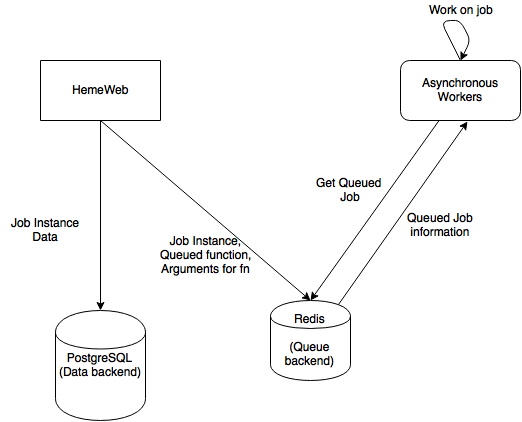
\includegraphics[keepaspectratio=true,scale=0.5]{../resources/images/hemeweb_master_components.png}
 }
\captionof{figure}{HemeWeb architecture}\label{fig:hemeweb-components}%      only if needed  
\end{minipage}

\vspace{1cm}

Figure \ref{fig:hemeweb-components} above illustrate how HemeWeb  application process interacts with the other components inside the master instance. It also illustrates how user's HTTP request start a chain of events inside the master master instance that will eventually return a response to the user's browser.

To start, user's browser will send an HTTP request to the master instance. This request will be captured by Nginx process that will act as a reverse proxy.  Nginx\footnote{\url{https://www.nginx.com}} will proxy the HTTP request towards the correct web application server process or serve static files depending on the requested URL. If the request is routed to the web application, HemeWeb web application which is handled by green unicorn\footnote{\url{http://gunicorn.org}} HTTP server will accept the request. This library will run the HemeWeb python code to process the HTTP request by the user. Depending on the type and path of the request, the web application will serve a static HTML as a response, or handle job-related logic that might interact with another part of the system. One of the components the web application might interact with is the PostgreSQL database\footnote{\url{https://www.postgresql.org}}. The database will persist job information locally on the instance to provide persistent information between HTTP request. However, it will be wiped out when the master instance is terminated and is not shared between HemeWeb instances.

Another part of the master instance the HemeWeb application can interact is with the queuing system. HemeWeb can submit a job into the queue which uses Redis datastore\footnote{\url{http://redis.io}} as the queue backend. HemeWeb uses third party library called Django-rq that handles asynchronous background tasks handling using Redis backend. It uses the pub / sub mechanism of Redis to create a lightweight background job workers. HemeWeb process will store the function to be executed, the job instance and parameters to used by the function into the Redis backend. A background worker will look at the queue at an interval and work on a job if there's any in the queue. The worker will execute the function and update the instance with relevant job execution result. Finally, the worker will go back to being idle waiting for next job to be executed.

\subsubsection{Docker components}

\vspace{1cm}

\noindent%
\begin{minipage}{\linewidth}% to keep image and caption on one page
\makebox[\linewidth]{
  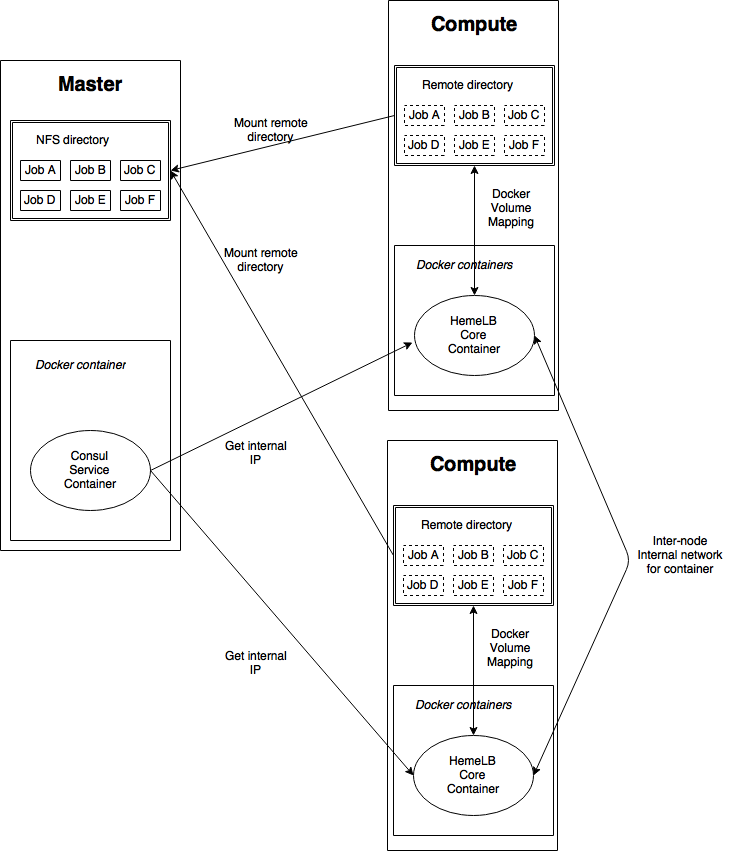
\includegraphics[keepaspectratio=true,scale=0.5]{../resources/images/hemeweb_docker.png}
 }
\captionof{figure}{HemeWeb Docker component}\label{fig:hemeweb-docker}%      only if needed  
\end{minipage}

\vspace{1cm}

In this section, I will discuss the interaction between Docker components and the hosts. As illustrated on figure \ref{fig:hemeweb-docker}, each host will run Docker service to run specific Docker container depending on their purpose.

In the master instance, a consul container is constantly running to provide inter-container communication mechanism. Consul\footnote{\url{https://www.consul.io}} is used by the Docker containers to coordinate the internal networking communication between them. In a host, multiple containers can be started without conflicting IP because they can communicate via the host. However, in HemeWeb the communication between containers will go beyond single hosts. Containers will need to communicate with other containers living on other hosts. Consul service is needed to coordinate this communication.

On the other hand, on the compute nodes, only HemeLB core container is run. The compute nodes will be started by a job submission to HemeWeb. After the nodes are started, HemeWeb process will instruct the compute nodes to pull the specified HemeLB core container version from Docker hub. If the specified version is locally cached on the compute nodes, no network activity will be made. HemeLB core container is then started to accept simulation command.

To start the simulation, the HemeLB core containers requires the job directories to be exported via Networked File System interface. HemeWeb process in the master node will prepare the job directories with the correct folder and files locally in the master node. Every job submission to HemeWeb will create a specific folder for storing submitted job-related files. The exported job directories will then be mounted by the compute nodes provisioned for the simulation. Finally, HemeLB simulation can use the mounted job directories to read input from and write output to.


\subsubsection{Job instance structure}

As mentioned above, HemeWeb uses Django web framework to handle web functionalities. Django framework follows the object-oriented principle where everything is modeled as an object. Job information that is handled by HemeWeb is also modeled as an object that is derived from object class of Django. Literally named \textbf{Job}, is a class that represents simulation information. Each instance of this class will contains information specific to a simulation instance. \textbf{Job} class inherits from \textit{django.db.models.Model} class that is included within Django framework. HemeWeb \textbf{Job} class extends this basic class and add functionalities specifically related to job information.


HemeWeb's Job class has the following attributes:
\begin{itemize}
    \item id:  This is a unique UUID field that represents the Job ID. UUID field was chosen because it is appropriate for the possibility of sharing the job simulation files between different deployment of HemeWeb. UUID can prevent clashes of job ID between these instances.
    \item input\_file, stl\_file, profile\_file, output\_file, configuration\_file:  These attributes keep track of the files that are used by the job. It is stored as the path to the file in the local filesystem, but with Django functionalities, HemeWeb can work with the file as an object.
    \item container\_image:  This attribute determines which container of HemeLB core will be used in the simulation. Currently, the choice of the field's value is set manually in the codebase. 
    \item instance\_type: This determines which compute node type will be started for the simulation. 
    \item instance\_count: This attribute determines how many compute node will be started for the simulation. Currently, this is also set manually in the source code. 
    \item status: The attribute to determine Job's status, whether it is \textit{queued, added, done, failed, etc}
    \item created: Attribute to keep track when the job is created
    \item updated: Attribute to keep track when the job is updated 
\end{itemize}



\subsubsection{Job directory structure}

Each simulation done with HemeWeb have its own job directory. These directories are located in the master instance and are shared with the compute node. To provide a clearer picture how the application package and work with the job's files, I will discuss how HemeWeb structure each job's files.


\begin{lstlisting}[numbers=none]
<UPLOAD_FOLDER_DIR>/<JOB_ID>
<UPLOAD_FOLDER_DIR>/<JOB_ID>/inputs/*
<UPLOAD_FOLDER_DIR>/<JOB_ID>/logs/*
<UPLOAD_FOLDER_DIR>/<JOB_ID>/outputs/*
<UPLOAD_FOLDER_DIR>/<JOB_ID>/metadata
\end{lstlisting}

Listing above illustrates the structure of a job instance's directory structure.  The first component of all job instance's directory is the UPLOAD\_FOLDER\_DIR. This is the path to a directory in which HemeWeb will upload all files. To change this parameter, one should change the path in the HemeWeb settings file and restart the web application so the changes took place.

The next part of the directory structure is the job folder named with its ID. The ID will be generated by HemeWeb using Universally Unique Identifier (UUID) scheme. More specifically, UUID Version 4 that depends on the random number. Using UUID is important for HemeWeb because it is accurately approximated to have a really low chance of producing duplicate ID. Hence, HemeWeb does not have to take care of the possibility of jobs having duplicate ID.

Next, we have the inputs folder inside the job folder. This is where all the inputs and configurations are stored by the web application. There's also logs folder, where the job stdout, stderr, and HemeLB logs are stored. The web application will read from this folder and make it available on the web interface. Outputs folder will be used by the HemeLB simulation to write output files in this folder. One final file is the metadata file. This file is used by the web application to store the state of the job. The job is pickled into this metadata file so when it is downloaded, the web application can unpickle the state of the job instance and it is preserved, ready to be used for another simulation.

A Job instance is preserved with this job directory structure. This allows job information to be preserved in an external storage that can be used for backup. HemeWeb currently supports uploading job directory to amazon simple storage service (S3). However, backup is not the only purpose for this functionalities. By making job directory files available to the public, independent peers can download these files and run the simulation with correct files and configurations. It allows peers to replicate a simulation exactly or with modifications.

\subsection{Simulation workflow}

\vspace{1cm}

\noindent%
\begin{minipage}{\linewidth}% to keep image and caption on one page
\makebox[\linewidth]{
  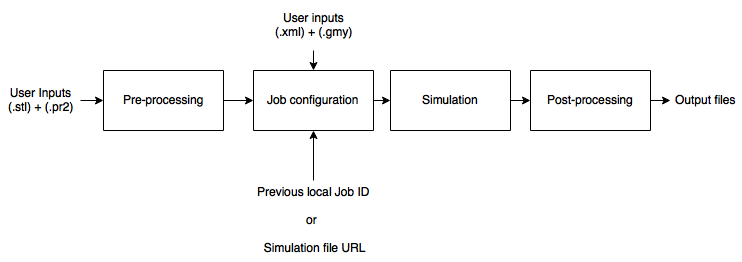
\includegraphics[keepaspectratio=true,scale=0.5]{../resources/images/implementation.png}
 }
\captionof{figure}{HemeWeb flow}\label{fig:hemeweb-implementation}%      only if needed  
\end{minipage}

\vspace{1cm}

Figure \ref{fig:hemeweb-implementation} illustrates how the HemeWeb web application works. HemeWeb currently consists of 4 core activities that will be discussed in details in the following section.

\subsubsection{Pre-processing}

In this step, HemeWeb handles pre-processing of inputs that are needed so that HemeLB simulation can parse the files. The user provides a geometry file (.stl) and a profile file (.pr2) to the web application for processing. HemeWeb will then create a job instance with these two files, save them locally on master instances and queue the pre-processing job.


\vspace{1cm}

\noindent%
\begin{minipage}{\linewidth}% to keep image and caption on one page
\makebox[\linewidth]{
  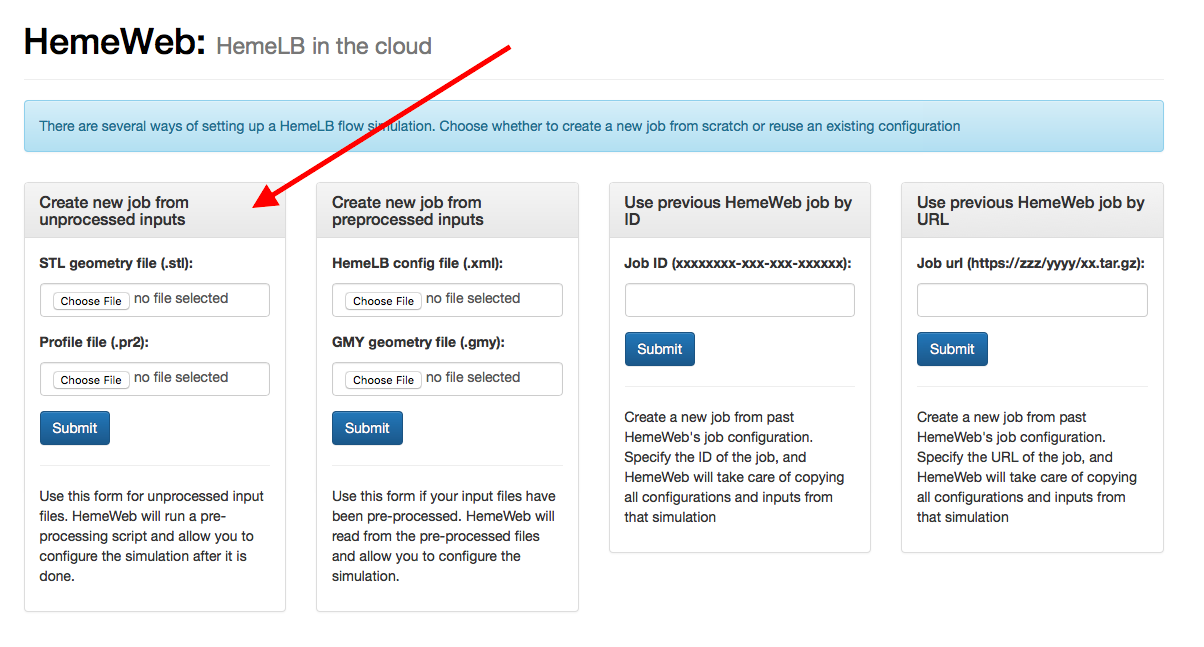
\includegraphics[keepaspectratio=true,scale=0.4]{../resources/images/pre-processing}
 }
\captionof{figure}{HemeWeb pre-processing form}\label{fig:hemeweb-pre-processing}%      only if needed  
\end{minipage}

\vspace{1cm}


Figure \ref{fig:hemeweb-pre-processing} shows HemeWeb user interface to upload the unprocessed files.  After submission of both files and job being queued, the asynchronous worker on the master instance will work on the job whenever they are free. It will run the pre-processing python script to generate the geometry files and HemeLB configuration file. These files will then be saved to the master instance, and HemeWeb will track these files by recording the path to these files on the job instance. Now the job instance is ready for the next step. of the workflow.

\subsubsection{Job configuration}

In this step, HemeWeb application will take a job instance with correctly set geometry file (.gmy) and HemeLB configuration (.xml). However, there are multiple ways that HemeWeb can get this correctly set job instance. As illustrated on Figure \ref{fig:hemeweb-implementation} , there are 4 possible entry points for this step. The web interface for these 4 entry points are also shown on Figure \ref{fig:hemeweb-pre-processing} They are:

\begin{itemize}
    \item \textbf{From the post-processing step.}
    	These files are generated from the previous pre-processing step. The job instance is directly used in this step
    
    \item \textbf{User's provided geometry and configuration file.}
    	User have pre-processed their own file locally, or have their own geometry and configuration files available. HemeWeb will create a new job instance, save both files and keep them tracked with the job instance.
	
    \item \textbf{User's provided previous job ID.}
    	There are two possible case when user specify previous job ID. First, the previous job is available locally on the HemeWeb instance. Second, the previous job is cached on the persistent storage on the cloud vendor and are not available locally. HemeWeb will download the previous file from the persistent storage if it is not available locally. It will then create a new job instance that copy the previous job's geometry file and configuration file to be used for further configuration.
    
    \item \textbf{User's provided simulation file URL.}
    	The last alternative is for user to provide the simulation file URL. Simulation files are uploaded to a persistent storage at the end of the workflow. These files, if made public, can be used by other instance of HemeWeb to download the simulation files and use it as a basis to create a new job instance. The way the system work is the same as using previous job ID, but its source is not its own persistent storage, but other people's simulation files.

\end{itemize}


After the job instance is created from one of the four way possible discussed above, HemeWeb will then ask users for the job configuration. 

\vspace{1cm}

\noindent%
\begin{minipage}{\linewidth}% to keep image and caption on one page
\makebox[\linewidth]{
  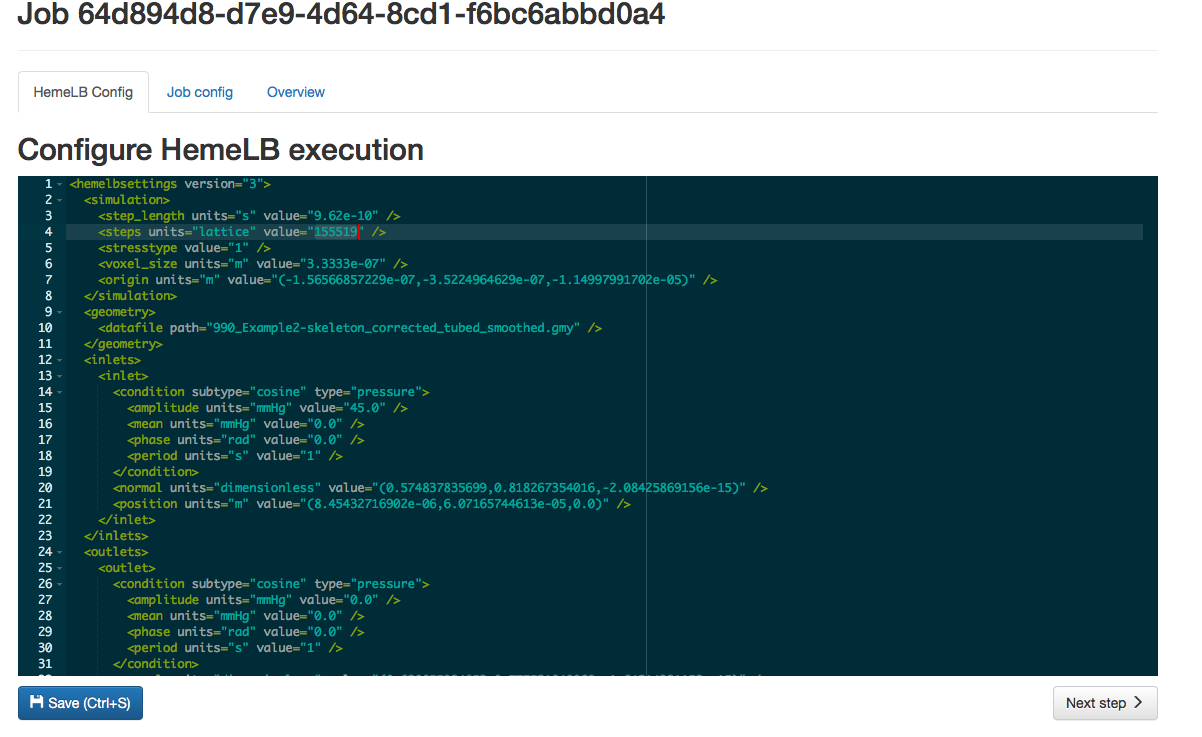
\includegraphics[keepaspectratio=true,scale=0.3]{../resources/images/configure1}
 }
\captionof{figure}{HemeWeb HemeLB configuration form}\label{fig:hemeweb-configure1}%      only if needed  
\end{minipage}

\vspace{1cm}

Figure \ref{fig:hemeweb-configure1} shows the interface where users are asked to configure the HemeLB simulation parameter. In this page, an online XML editor will be provided for the user to directly edit the .xml file that is provided by the users or from the  pre-processing step. Users can directly edit values that affect simulation execution like inlet pressure, outlet pressure, blood viscosity, and etc. After configuring the simulation parameter it will then be redirected to job configuration page.



\vspace{1cm}

\noindent%
\begin{minipage}{\linewidth}% to keep image and caption on one page
\makebox[\linewidth]{
  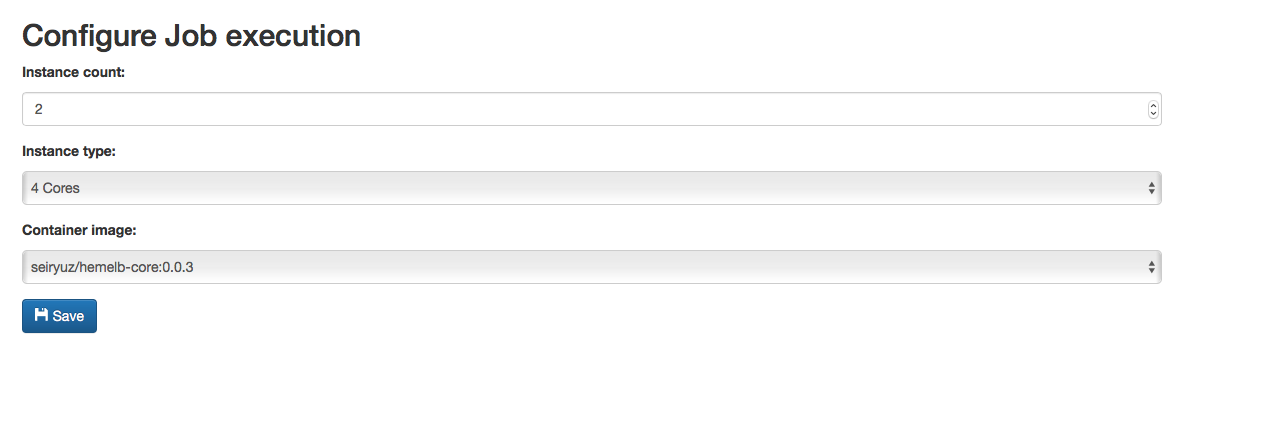
\includegraphics[keepaspectratio=true,scale=0.3]{../resources/images/configure2}
 }
\captionof{figure}{HemeWeb Job configuration form}\label{fig:hemeweb-configure2}%      only if needed  
\end{minipage}

\vspace{1cm}

Figure \ref{fig:hemeweb-configure2} shows the job configuration page. This page asks users about the parameter in which the simulation will be run with. These parameters are instance count, instance type, and HemeLB core container version. Instance count will determine how many compute node will be provisioned for this simulation by HemeWeb. Instance type will determine what type of compute node will be started, and the HemeLB core container version will determine what version of the container the compute node will use to run HemeLB simulation. After all of these parameters are set, users will be asked to confirm the job execution in the overview page. In the page, the user can then finally queue the job into the queue system.



\subsubsection{HemeLB simulation}

Once job instance is queued into the simulation queue, a free asynchronous worker will pop the queue and run the job. The worker will start up the configured amount and type of server instance from the cloud provider. These instances will then be further reconfigured by an ansible script so that it points to the correct master instance address. Next, input files are shared via Networked File System(NFS), the compute units will mount the input folders to their instance. 

The correct HemeLB core container version will be pulled from Docker hub in the next step. This step will skip the download if the container asked are already cached in the image for compute units which are prepared on the deployment part. After all of these are done, then the simulation can finally begin. Master node will issue an MPI command to be run by the leader of compute nodes. The leader of compute node then will run this MPI command in the Docker container. This command will be run on multiple compute node if it is configured as such in the previous steps. 

The HemeLB simulation will run until outputs are produced. The output will be written back to the correct output folder in the shared folder. This means that the master instance will have access to the outputs file and can do further processing. This step ends with the termination of the instances.

\vspace{1cm}

\noindent%
\begin{minipage}{\linewidth}% to keep image and caption on one page
\makebox[\linewidth]{
  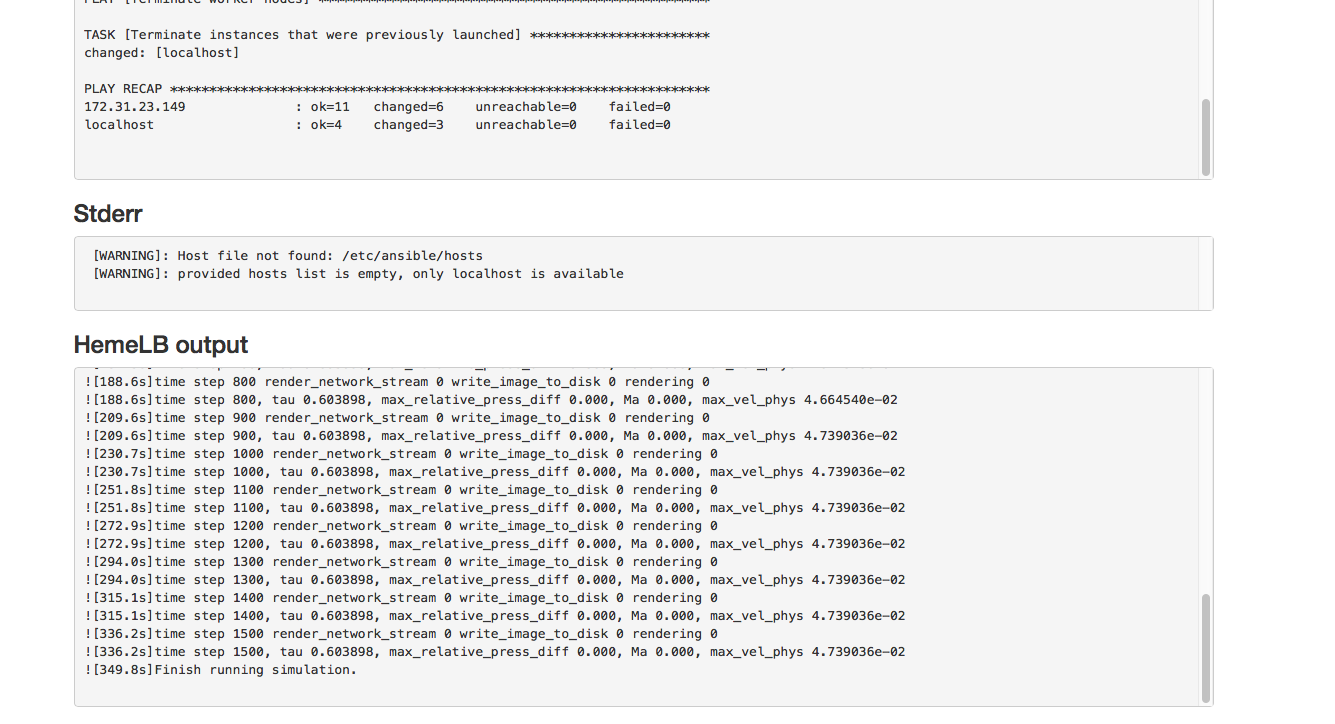
\includegraphics[keepaspectratio=true,scale=0.3]{../resources/images/output}
 }
\captionof{figure}{HemeWeb Job logs}\label{fig:hemeweb-output}%      only if needed  
\end{minipage}

\vspace{1cm}

Figure \ref{fig:hemeweb-output} shows how the Job execution will produce logs that can be viewed on HemeWeb web application. During simulation, logs are written to the respective job folder and are served to the browser by the HemeWeb app. Showing the logs allows users to easily view the progress of the job or even debug failed job.


\subsubsection{Post-processing}

After HemeLB simulation is finished, HemeWeb web app will do some post-processing steps to make sure the output files can be viewed easily. The outputs from HemeLB simulation are structured in such a way that makes it efficient to write in parallel. However, these outputs cannot be viewed by visualization system like Paraview. What HemeWeb will do is to pipe the output files to two python scripts that will format the output into a format that can be understood by ParaView.


However, the post-processing steps are not done yet. There are further steps that HemeWeb took to make sure that the simulation files, configurations, and results are preserved externally. HemeWeb will package the job directory, compressed it, and upload it into persistent storage that cloud vendors provide. As the time of writing, HemeWeb only supports amazon simple storage service. The simulation files are uploaded to this storage and made accessible to the public so other HemeWeb instance can use them. Also, with the job files persisted on persistent storage, the next HemeWeb instance deployed can take advantage of these files that it can use it as previous jobs to be used on current deployment





\subsection{Implementation Challenge}


In this section, I will try to outline and discuss the challenges in implementing this project, and if any, the solution that I choose.

\subsubsection{Cloud vendors features and API difference}

The challenge in developing the deployment script is the difference of cloud vendors' API and features.  This has led to some problems when trying to create a common API to do a certain task. One notable problem is that the absence of image creation from running instance feature from one of the cloud vendors. Image creation feature is not an essential requirement of the project. However, with an image creation, the compute nodes that will be requested by the web application can be configured much quicker because all the pre-configuration that are done during the deployment phase. However, one of the cloud vendors does not have this feature. This creates a situation where there is no elegant way to create image with the deployment script and users are asked to manually created the image on the web interface

\vspace{1cm}

\noindent%
\begin{minipage}{\linewidth}% to keep image and caption on one page
\makebox[\linewidth]{
  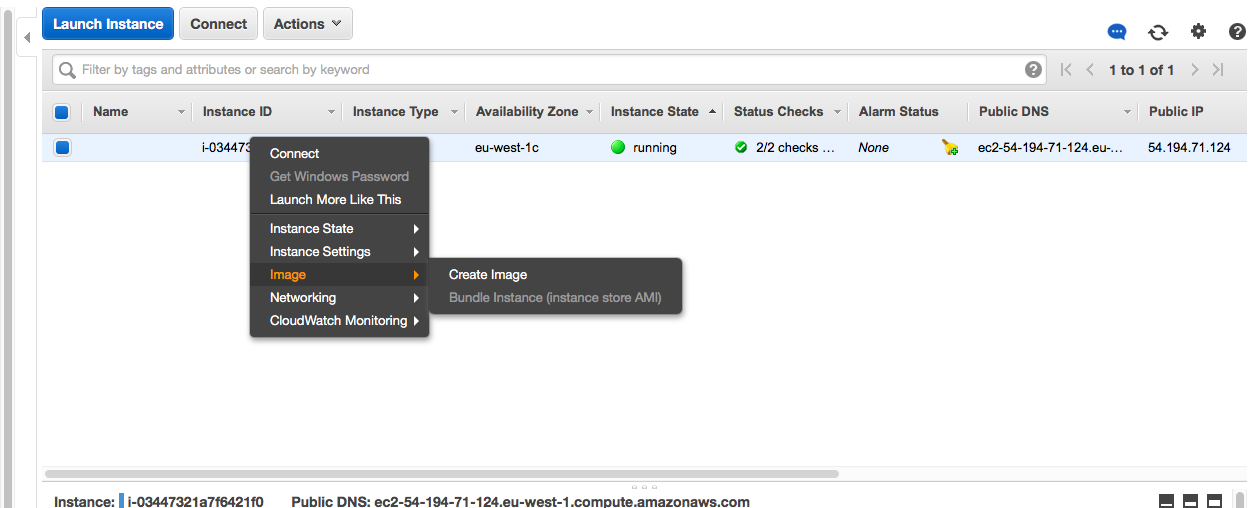
\includegraphics[keepaspectratio=true,scale=0.4]{../resources/images/hemeweb-challenge-1.png}
 }
\captionof{figure}{Manual image creation instead of automatic}\label{fig:hemeweb-challenge-1}%      only if needed  
\end{minipage}

\vspace{1cm}

Figure \ref{fig:hemeweb-challenge-1} shows how users are instructed to manually create an image from running instance. Users have to go the web interface of specific cloud vendors, right-click on the running instance, and create the image from it. This is a simple workaround which is less complicated compared to accommodating different or missing features and API from different cloud vendors.


Another problem is the time constraint. Due to the time constraint, I cannot achieve full compatibility with all cloud vendors. The development time is mainly focused on amazon web service because it has all the features HemeWeb need. However, this means that the codebase is currently tied to one cloud vendors. Features like automatically reading past simulation files from cloud storage and uploading simulation files are tied to amazon infrastructure. It is possible to refactor these functionalities out to become more generic, however for the interest of time, I decided not to.

\subsubsection{Security}

Another challenge that I face during the development of HemeWeb is to handle the security of the application. However, security is not the main focus of this work and is apparent in the development of the application. I will still discuss the security issues so that I can give an objective assessment of the application.

The first security issues that I found is with regards to the compute node security in some cloud vendors. Digital ocean, for example, does not provide a "real" private networking option within compute nodes. They have a "shared" private networking options that allow other compute nodes, which are not even on your account have network connectivity to your node. Theoretically, this allow other people access to your private compute node if they have the credentials. In this case, I made sure that all the compute nodes have a sensible access policy to deter unauthorized access to the nodes. I only allow ssh with a public key and disabled password access to ssh. Also, it is also much better to choose cloud vendors that have real private networking like AWS. In which, the compute nodes are not accessible to other nodes that are not part of your own private network. This is much more secure and sensible.


Another security issue is on how compute and master node share simulation job's files. It currently uses Network File System without any security measures towards the nodes that try to mount it via the private network. There is an opportunity to secure this communication by encrypting the job files, but it is not currently done.


\section{Development process}

The development process is divided into 5 phases. The planned phases are as follow:

\begin{enumerate}
    \item{Separate HemeLB core into its own container}
    \item{Orchestrate the deployment of HemeLB cluster / infrastructure}
    \item{Develop HemeWeb to accept user input}
    \item{Extends HemeWeb to handle geometry generation workflow}
    \item{Extends HemeWeb to handle domain definition step or Viewing of HemeLB simulation result}
\end{enumerate}

The development process loosely follows the agile method in which I regularly meet with the stakeholders every week to give an update and gather feedback on the project. The phases are designed in such a way to minimize the risk of having nothing at all during the end of the project phase. This is due to that HemeWeb can work on its own after finishing step 3. The HemeLB simulation can be done on its own. The rest of the steps are there to extend the functionalities of the HemeWeb to cover more functionalities.

During the first week of the development, I focused more on stripping the HemeLB core container into its own. I researched on how Docker and Dockerfile work, and finding out what are the issues with the current container. After identifying the issues, which are ssh service and full of functionalities which are not essential, I stripped down the image and changed the base image so that the container could avoid the mentioned problems. I end up with smaller container size and it is available online on https://hub.docker.com.

However, one particular issue with what I have currently is that the Dockerfile is published as a part of the HemeWeb source code. It should be tied down to the HemeLB development instead of HemeWeb. Currently, the development model of HemeLB is that there is an internal private repository where the less than stable build is pushed to it, and there are public repositories where only stable builds are pushed into. The release process should include adding the Dockerfile towards the core HemeLB source code repository and tagging the release correctly. HemeLB core containers should then be built automatically on Docker hub with regards to additional tags being pushed to the public repository.


After the development of HemeLB core container, I then focused on how the architecture could be primed for the HemeLB simulation. It involves on configuring the servers and all supporting infrastructures on cloud vendors to be ready for HemeLB simulation. Network configuration, security configuration, Docker configuration, and other should be handled automatically. I elect to choose ansible orchestration software because it is closely related to python language that I used. 

In this phase, I successfully achieve the provision and deployment process that with the correct credentials and authorization, the script could provision and configure the architecture correctly so it is ready for HemeLB simulation. In addition to that, I successfully created the script so that it will be cloud vendors agnostic. I can deploy the architecture to google cloud vendors, amazon web service, and digital ocean.

However, it is to be noted that the deployment process that I achieve can only run HemeLB simulation from the command line. I have not considered the web application installation and configuration at this point of the deployment. I only considered the infrastructure being built and configured for HemeLB simulation.


Next, I started developing HemeWeb web application. I choose Django web application framework due to my experience with it. I created a basic interface, where job simulation is listed on the index page on the home interface. After that, I added a basic interface to add new job with a geometry file and HemeLB configuration file. The web application will then add those input files into a newly created job instance and configure the job instance in the job configuration step. The job will then be submitted. 

Here I developed a separate ansible script that will be called when a queued job is being worked at. The ansible script is responsible for starting up compute nodes needed by the job and executing HemeLB simulation. After the simulation is done, the script is also responsible for correctly terminating the compute node.

After the basic HemeWeb web application is achieved, I extend it to handle pre-processing. I added an extra form in the adding new job form to handle a profile file and geometry file. These two files will be converted into a geometry file and HemeLb configuration file that the job configuration steps expect. In addition to adding the interface, I also added a new function on the job instance that will run this pre-processing step on the background. 

Lastly, due to the limited time, I can only manage to run a small post-processing step on HemeWeb. What I did was adding post-processing step that converts the Extracted results from HemeLB output into a format that can be viewed by third party software, ParaView. The results are piped into two scripts that will output a .vtu that is compatible with ParaView. This is done during the background activity after simulation result is outputted. However, currently, this is done on the master node.

In addition to that, I also managed to add persistence capability to HemeWeb application. What I did was to package the job simulation folder into a compressed archive and upload it to persistent storage service of cloud vendors. These archives can be queried by another instance of HemeWeb to get previous job IDs available for the particular cloud vendor account used to deploy HemeWeb.  Also, the job simulation file URL is also showed on the web interface. Making it easy for the users to share the simulation file with their peers.




